\documentclass[oneside, 11pt]{article}

\usepackage[T1]{fontenc}
\usepackage[utf8]{inputenc}
\usepackage[dutch]{babel}

\usepackage{fouriernc}
\usepackage[detect-all, load-configurations=binary,
            separate-uncertainty=true, per-mode=symbol,
            retain-explicit-plus, range-phrase={ tot }]{siunitx}

\usepackage{setspace}
\setstretch{1.2}

\setlength{\parskip}{\smallskipamount}
\setlength{\parindent}{0pt}

\usepackage{geometry}
\geometry{marginparwidth=0.5cm, verbose, a4paper, tmargin=3cm, bmargin=3cm, lmargin=2cm, rmargin=2cm}

\usepackage{float}

\usepackage[fleqn]{amsmath}
\numberwithin{equation}{section}
\numberwithin{figure}{section}

\usepackage{graphicx}
\graphicspath{{Figures/}}
\usepackage{subfig}

\usepackage{tikz}
\usetikzlibrary{plotmarks}

\usepackage{fancyhdr}
\pagestyle{fancy}
\fancyhf{}
\rhead{\thepage}
\renewcommand{\footrulewidth}{0pt}
\renewcommand{\headrulewidth}{0pt}

\usepackage{relsize}
\usepackage{xspace}
\usepackage{url}

\newcommand{\figref}[1]{Figuur~\ref{#1}}

\newcommand{\hisparc}{\textsmaller{HiSPARC}\xspace}
\newcommand{\kascade}{\textsmaller{KASCADE}\xspace}
\newcommand{\sapphire}{\textsmaller{SAPPHiRE}\xspace}
\newcommand{\jsparc}{\textsmaller{jSparc}\xspace}
\newcommand{\hdf}{\textsmaller{HDF5}\xspace}
\newcommand{\aires}{\textsmaller{AIRES}\xspace}
\newcommand{\csv}{\textsmaller{CSV}\xspace}
\newcommand{\python}{\textsmaller{PYTHON}\xspace}
\newcommand{\corsika}{\textsmaller{CORSIKA}\xspace}
\newcommand{\labview}{\textsmaller{LabVIEW}\xspace}
\newcommand{\daq}{\textsmaller{DAQ}\xspace}
\newcommand{\adc}{\textsmaller{ADC}\xspace}
\newcommand{\adcs}{\textsmaller{ADC}s\xspace}
\newcommand{\Adcs}{A\textsmaller{DC}s\xspace}
\newcommand{\hi}{\textsc{h i}\xspace}
\newcommand{\hii}{\textsc{h ii}\xspace}
\newcommand{\mip}{\textsmaller{MIP}\xspace}
\newcommand{\hisparcii}{\textsmaller{HiSPARC II}\xspace}
\newcommand{\hisparciii}{\textsmaller{HiSPARC III}\xspace}
\newcommand{\pmt}{\textsmaller{PMT}\xspace}
\newcommand{\pmts}{\textsmaller{PMT}s\xspace}

\DeclareSIUnit{\electronvolt}{\ensuremath{\mathrm{e\!\!\:V}}}

\DeclareSIUnit{\unitsigma}{\ensuremath{\sigma}}
\DeclareSIUnit{\mip}{\textsmaller{MIP}}
\DeclareSIUnit{\adc}{\textsmaller{ADC}}

\DeclareSIUnit{\gauss}{G}
\DeclareSIUnit{\parsec}{pc}
\DeclareSIUnit{\year}{yr}



\begin{document}

\title{Inregelen \pmts}
\author{D. B. R. A. Fokkema}
\date{}

\maketitle

\section{Werking van een \pmt}

Een fotoversterkbuis (photomultiplier tube, of \pmt) is een
elektronenbuis die in staat is om hele kleine lichtflitsjes om te zetten
in een elektrisch signaal.  Het is zelfs mogelijk om afzonderlijke fotonen
te tellen.  Geladen deeltjes uit kosmische straling die door de \hisparc
detectoren gaan verliezen energie in het materiaal van de detectoren.  In
de scintillator wordt dat energieverlies omgezet in een zwak
lichtschijnsel.  Dit paarsblauwe licht verspreidt zich door de detector
weerkaatst zo veel mogelijk aan de randen en een deel komt terecht bij de
\pmt, die het licht detecteert en een signaal afgeeft aan de \hisparc
elektronica.

Een \pmt maakt gebruik van het fotoelektrisch effect.  Dit effect werd
verklaard door Einstein en hiervoor ontving hij in 1921 de
Nobelprijs.\footnote{Veel mensen gaan er van uit dat Einstein de Nobelprijs
ontving voor de relativiteitstheorie, maar dit klopt niet.}  Wanneer licht
op een metaal schijnt, kunnen er elektronen worden losgeslagen uit het
oppervlak.  Dit gebeurt wanneer de energie per foton hoger is dan de
energie die een elektron nodig heeft om los te komen uit het metaal.  Deze
drempelenergie is afhankelijk van het soort metaal.  De energie per foton
wordt gegeven door
\begin{equation}
E_f = \frac{hc}{\lambda},
\end{equation}
met $E_f$ de energie van het foton, $h$ de constante van Planck, $c$ de
lichtsnelheid en $\lambda$ de golflengte van het licht.  Zie ook Tabel 7
en Tabel 35 in je Binas.

De energie van een foton is dus omgekeerd evenredig met de golflengte:
$E_f \propto 1/\lambda$.  Hoe kleiner de golflengte van het licht, hoe
groter de energie per foton.  Dit betekent dat hoe `blauwer' het licht,
hoe makkelijker een elektron wordt losgemaakt.  Is het licht \emph{te}
`rood', dan lukt dat nooit.  Daarom hebben we een scintillator gekozen die
een violet licht uitstraalt.

\begin{figure}
\centering
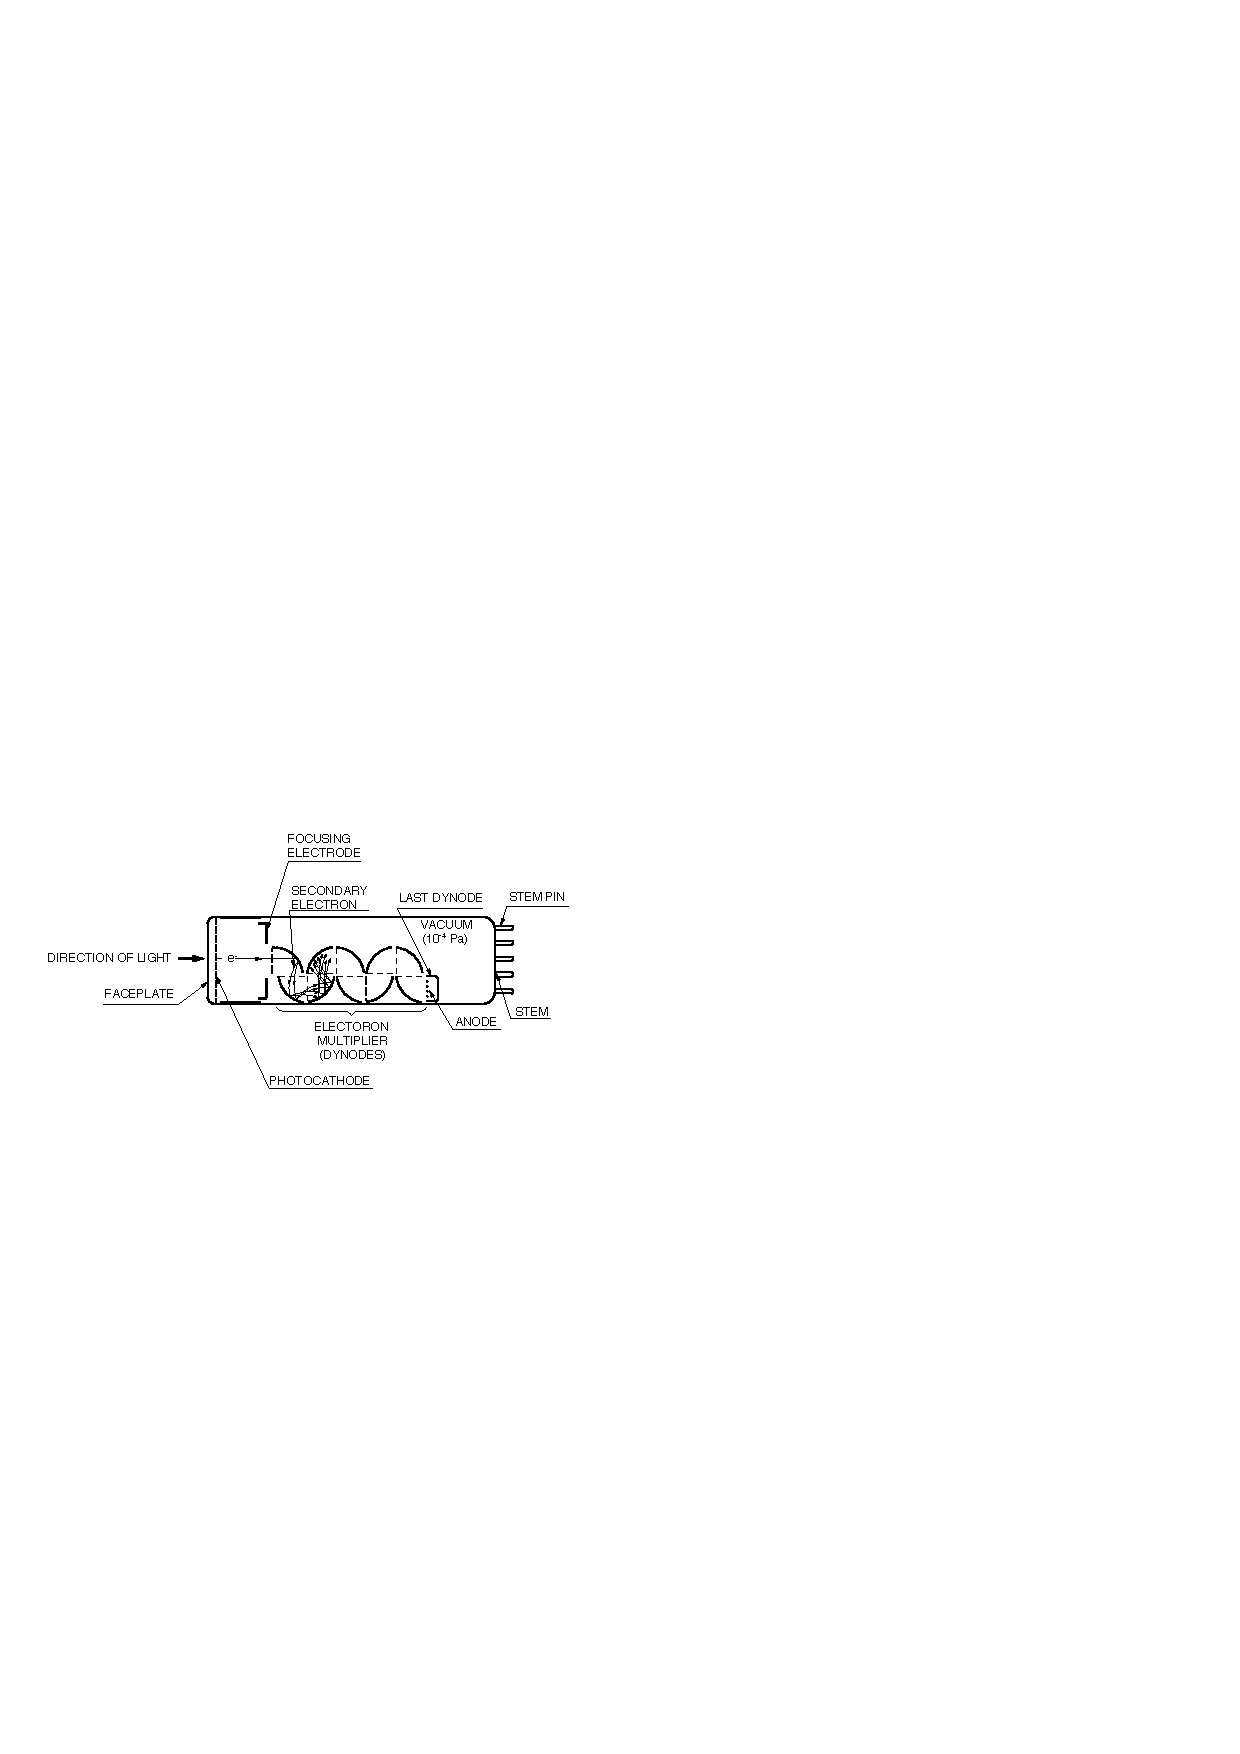
\includegraphics{pmt-schematic}
\caption{Schematische weergave van een \pmt.  Figuur overgenomen uit
\cite{hamamatsu}.}
\label{fig:pmt}
\end{figure}

De \pmt is een verzegelde glazen buis die vacuüm gemaakt
is\figref{fig:pmt}.  De voorkant van een \pmt bestaat uit een dunne
glaslaag.  Aan de binnenkant van het glas is een zeer dun metaallaagje
opgedampt.  Het laagje is zó dun, dat het doorzichtig is.  Licht dat op de
\pmt valt, gaat door het glas en raakt het metaal.  Het violette licht uit
de scintillator heeft een $E_f$ die hoog genoeg is om elektronen vrij te
maken uit het metaallaagje.  Om er voor te zorgen dat er veel elektronen
beschikbaar zijn wordt het metaalplaatje op een grote negatieve spanning
gezet.  De elektronen staan dan feitelijk te dringen om het metaal te
verlaten.  Het metaallaagje heet dan ook de \emph{kathode}\footnote{In een
vacuümbuis is de kathode de pool waar elektronen uit worden vrijgemaakt,
zoals hier gebeurt.} van de \pmt.  De \emph{anode} van de fotobuis wordt
geaard, waardoor er een sterk elektrisch veld in de buis ontstaat.  De
elektronen versnellen richting de anode.  Om een grote versterkingsfactor
te krijgen is de buis opgedeeld in meerdere trappen.  Iedere trap heeft
een \emph{dynode}, een metalen plaatje met een iets minder negatieve
spanning dan de voorgaande dynode.  Dus bij een \pmt met drie dynodes,
zijn de spanningen bijvoorbeeld als volgt: kathode (\SI{-1000}{\volt}),
eerste dynode (\SI{-750}{\volt}), tweede dynode (\SI{-500}{\volt}), derde
dynode (\SI{-250}{\volt}) en kathode (\SI{0}{\volt}).  Zo blijven de
elektronen versnellen van kathode, langs alle dynodes en uiteindelijk naar
de anode.  De versterking treedt op zodra de elektronen een dynode raken.
De grote snelheid waarmee een elektron het metaal intreedt maakt een
aantal elektronen los.  Deze losgeslagen elektronen worden vervolgens
versneld naar de volgende dynode.  Als per dynode per elektron
bijvoorbeeld drie elektronen worden losgeslagen, dan is de totale
versterking in een \pmt met tien dynodes gelijk aan $3^{10} \approx
\num{60000}$.  De hoogspanning die over de \pmt staat bepaalt in grote
mate de versterkingsfactor.  Hoe hoger de spanning, hoe groter de
versterkingsfactor.  De hoogspanning bepaalt namelijk enerzijds de
versnelling van de elektronen en anderzijds het aantal elektronen dat
staat te dringen om de dynode te verlaten.

De \pmt die gebruikt wordt door \hisparc is een 9107B van Electron
Tubes \cite{9107B}.  Deze heeft 11 dynodes en een typische versterking van
\num{3e6} bij \SI{850}{\volt}.  Dat komt overeen met $\num{3.9}^{11}$.  Voor
ieder elektron dat een dynode raakt worden er gemiddeld bijna vier
elektronen vrijgemaakt.


\section{Signaal uit \hisparc detectoren}

Het signaal uit de \pmt wordt via kabels met een lengte van
\SI{30}{\meter} naar de \hisparc elektronica geleid.  Alle kabels zijn
precies even lang, om te zorgen dat het signaal uit alle detectoren op
hetzelfde moment bij de elektronica aankomt.  Zodra een air shower een
detector bereikt gaan één of meerdere deeltjes door de detector.  Dit
veroorzaakt een pulsvormig signaal.  De relatief lange staart van het
signaal wordt veroorzaakt door licht dat via een aantal reflecties alsnog
bij de \pmt terecht komt, maar ook door deeltjes die een beetje
achterliepen in de shower en vrij laat door de detector gaan.  In
\figref{fig:traces} staat het signaal van een \hisparc event.  Het bestaat
uit een flinke puls met wat kleinere pieken in de staart.  Dit signaal is
veroorzaakt door meerdere deeltjes die (vrijwel) gelijktijdig door de
detector gingen.  De eerste grote puls is een optelsom van het licht van
meerdere deeltjes.

Als je alle signalen uit een \hisparc detector bekijkt, dan zie je grote
verschillen.  Dit komt een event veroorzaakt kan worden door één, twee,
drie, of zelfs méér geladen deeltjes die door de detector gaan.  Ook
ontstaan er hoogenergetische fotonen in air showers.  Deze fotonen geven,
met een kleine kans, een relatief zwak signaal in de detectoren.  Maar
omdat het aantal fotonen in een air shower enorm groot is zie je dit terug
in signalen uit de \hisparc detectoren.




\begin{figure}
\centering
\documentclass[oneside, 11pt]{article}

\usepackage[T1]{fontenc}
\usepackage[utf8]{inputenc}
\usepackage[dutch]{babel}

\usepackage{fouriernc}
\usepackage[detect-all, load-configurations=binary,
            separate-uncertainty=true, per-mode=symbol,
            retain-explicit-plus, range-phrase={ tot }]{siunitx}

\usepackage{setspace}
\setstretch{1.2}

\setlength{\parskip}{\smallskipamount}
\setlength{\parindent}{0pt}

\usepackage{geometry}
\geometry{marginparwidth=0.5cm, verbose, a4paper, tmargin=3cm, bmargin=3cm, lmargin=2cm, rmargin=2cm}

\usepackage{float}

\usepackage[fleqn]{amsmath}
\numberwithin{equation}{section}
\numberwithin{figure}{section}

\usepackage{graphicx}
\graphicspath{{Figures/}}
\usepackage{subfig}

\usepackage{tikz}
\usetikzlibrary{plotmarks}

\usepackage{fancyhdr}
\pagestyle{fancy}
\fancyhf{}
\rhead{\thepage}
\renewcommand{\footrulewidth}{0pt}
\renewcommand{\headrulewidth}{0pt}

\usepackage{relsize}
\usepackage{xspace}
\usepackage{url}

\newcommand{\figref}[1]{Figuur~\ref{#1}}

\newcommand{\hisparc}{\textsmaller{HiSPARC}\xspace}
\newcommand{\kascade}{\textsmaller{KASCADE}\xspace}
\newcommand{\sapphire}{\textsmaller{SAPPHiRE}\xspace}
\newcommand{\jsparc}{\textsmaller{jSparc}\xspace}
\newcommand{\hdf}{\textsmaller{HDF5}\xspace}
\newcommand{\aires}{\textsmaller{AIRES}\xspace}
\newcommand{\csv}{\textsmaller{CSV}\xspace}
\newcommand{\python}{\textsmaller{PYTHON}\xspace}
\newcommand{\corsika}{\textsmaller{CORSIKA}\xspace}
\newcommand{\labview}{\textsmaller{LabVIEW}\xspace}
\newcommand{\daq}{\textsmaller{DAQ}\xspace}
\newcommand{\adc}{\textsmaller{ADC}\xspace}
\newcommand{\adcs}{\textsmaller{ADC}s\xspace}
\newcommand{\Adcs}{A\textsmaller{DC}s\xspace}
\newcommand{\hi}{\textsc{h i}\xspace}
\newcommand{\hii}{\textsc{h ii}\xspace}
\newcommand{\mip}{\textsmaller{MIP}\xspace}
\newcommand{\hisparcii}{\textsmaller{HiSPARC II}\xspace}
\newcommand{\hisparciii}{\textsmaller{HiSPARC III}\xspace}
\newcommand{\pmt}{\textsmaller{PMT}\xspace}
\newcommand{\pmts}{\textsmaller{PMT}s\xspace}

\DeclareSIUnit{\electronvolt}{\ensuremath{\mathrm{e\!\!\:V}}}

\DeclareSIUnit{\unitsigma}{\ensuremath{\sigma}}
\DeclareSIUnit{\mip}{\textsmaller{MIP}}
\DeclareSIUnit{\adc}{\textsmaller{ADC}}

\DeclareSIUnit{\gauss}{G}
\DeclareSIUnit{\parsec}{pc}
\DeclareSIUnit{\year}{yr}



\title{Pulshoogte en pulsintegraal}
\author{N.G. Schultheiss}
\docwerkblad{2}{PH}
\version{1.0}

\begin{document}

\maketitle

\section{Inleiding}

Elke detector van een \hisparc-station is uitgerust met een
foto-versterker buis (PhotoMultiplier Tube: \pmt). Als er geen deeltjes
door de detector schieten, treedt er geen fluorescentie in de detector
op en ontstaat er geen licht. In dit geval geeft de PMT-buis een
elektrisch signaal van \SI{0}{\milli\volt} aan de \hisparc unit. Als er
wel deeltjes door de detector schieten, treedt er fluorescentie in de
detector op en ontstaat er licht. Dan geeft de PMT-buis een elektrisch
signaal af waarvan het aantal mV afhangt van het aantal deeltjes dat
door de detector is gegaan. In de \hisparc unit wordt het analoge
signaal door middel van een Analoog Digitaal Converter (\adc) omgezet in
een digitaal signaal. De grootte van dit signaal wordt uitgedrukt in
\adcs, de \adc count (een getal zonder eenheid).

Als er een detectorsignaal gemeten wordt, wordt een reeks van deze \adcs
in de \hisparc unit opgeslagen. Als er tegelijkertijd een tweede reeks,
van een andere detector, wordt opgeslagen, worden alle reeksen \adcs van
de \hisparc unit naar de \hisparc server gezonden. Met dergelijke reeks
kan een diagram van het verloop van het signaal tegen de tijd worden
gemaakt. In deze diagrammen zijn van het negatieve maximale signaal de
pulshoogte en het oppervlak, de pulsintegraal, te bepalen. Gedurende de
dag worden alle pulshoogten en pulsintegralen van een station verzameld.
Pulshoogte en pulsintegraal histogrammen zijn op te vragen op:
\url{http://data.hisparc.nl/} door op de stationsnaam te klikken.
Rechtsboven beide histogrammen is een link waarmee de gegevens in een
spreadsheet, zoals Excel, te laden zijn.


\section{De pulsvorm}


\subsection{Pulsen ophalen uit de \hisparc data opslag}

\begin{figure}[ht]
    \centering
    \subfloat{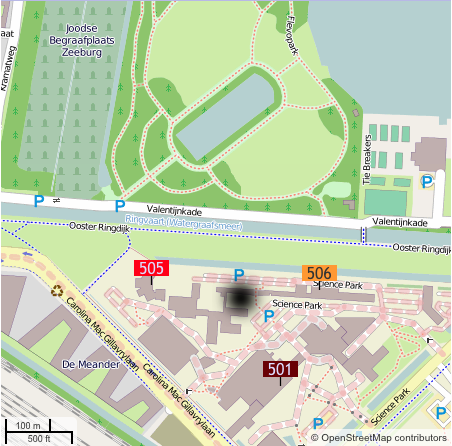
\includegraphics[scale=0.33]{kaart}}
    \subfloat{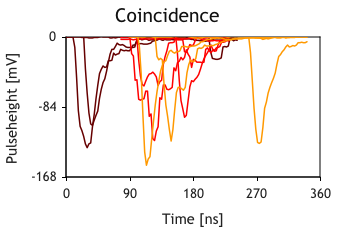
\includegraphics[scale=0.65]{Coincidence}}
    \caption{De plattegrond met de locaties van de meetstations
             en de gemeten pulsen per station.}
    \label{fig:coincidence}
\end{figure}

In de praktijk kunnen we een set pulsen voor een willekeurige
gebeurtenis ophalen met \jsparc%
\footnote{Het interactieve practicum \jsparc kan in de les na aanvraag
van een sessie worden gebruikt, het is ook mogelijk om een willekeurige
set pulsen op te halen op:
\url{http://data.hisparc.nl/media/jsparc/jsparc.html}.%
}. In deze module gaan we uit van de set pulsen die met de stations
uit \figref{fig:coincidence} zijn gemeten.

Op de kaart zijn drie meetstations te zien, een bruin, een rood en een
oranje station%
\footnote{De kleuren van de stations volgen de definitie van de
kleurcode van weerstandjes: bruin: 1, rood: 2, oranje: 3, geel: 4,
groen: 5, blauw: 6, violet: 7, etc. %
}. We zien dat alle stations meerdere pulsen hebben gegeven, dit komt
omdat een station uit meerdere detectoren bestaat. De hoogtes van de
pulsen zijn vergelijkbaar, bijgevolg is het midden van de air-shower
(zwarte vlek in \figref{fig:coincidence}) even ver van alle stations.


\subsection{Eenvoudige pulsvormen}

Het is mogelijk om de diagrammen per detector van een enkel station
te bekijken. In \figref{fig:Eenvoudige-pulsen} zijn de signalen
van vier detectoren van Station 506 te zien. De zwarte puls van detector
1 heeft een vrij steile voorflank. Het verloop van de achterflank
lijkt een halfwaardetijd te hebben (deze loopt exponentieel op). Bij
de blauwe grafiek van detector 4 is iets soortgelijks aan de hand.
Een deeltje lijkt dus herkend te worden aan een steile dalende flank
die wordt gevolgd door een exponentieel oplopende achterflank.

\begin{figure}[ht]
    \centering
    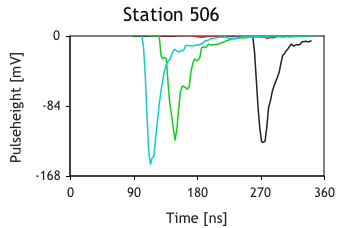
\includegraphics[scale=0.65]{Traces506}
    \caption{Eenvoudige pulsen}
    \label{fig:Eenvoudige-pulsen}
\end{figure}


\begin{minipage}[t]{1\columnwidth}%

\paragraph{Opdracht 1:}

De groene grafiek van detector 3 in \figref{fig:Eenvoudige-pulsen}
heeft een minder vloeiend verloop. Stel een hypothese op waarmee dit
minder vloeiende verloop kan worden verklaard.

\begin{center}
    \rule{\textwidth}{0.3mm}\\
    \rule{\textwidth}{0.3mm}\\
    \rule{\textwidth}{0.3mm}\\
    \rule{\textwidth}{0.3mm}\\
\end{center}
\end{minipage}

\bigskip{}


Meestal zien de grafieken er niet zo mooi uit als in
\figref{fig:Eenvoudige-pulsen}. In \figref{fig:Iets-complexere-pulsen}
zijn andere pulsen van detector 1 en 4 van Station 501 te zien
(respectievelijk zwart en blauw).

\begin{figure}[ht]
    \centering
    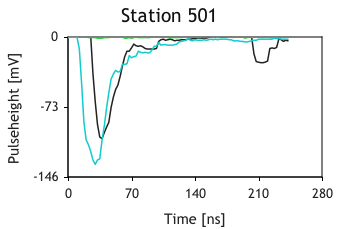
\includegraphics[scale=0.65]{Traces501}
    \caption{Iets complexere pulsen}
    \label{fig:Iets-complexere-pulsen}
\end{figure}


\begin{minipage}[t]{1\columnwidth}%

\paragraph{Opdracht 2:}

Geef een verklaring voor het verloop van de grafiek van detector
1 in \figref{fig:Iets-complexere-pulsen}.

\begin{center}
    \rule{\textwidth}{0.3mm}\\
    \rule{\textwidth}{0.3mm}\\
    \rule{\textwidth}{0.3mm}\\
    \rule{\textwidth}{0.3mm}\\
\end{center}
\end{minipage}

\bigskip{}


\begin{minipage}[t]{1\columnwidth}%

\paragraph{Opdracht 3:}

Bereken de afstand tussen de waargenomen deeltjes in de grafiek
van detector 1 (zwart) in \figref{fig:Iets-complexere-pulsen}.

\begin{center}
    \rule{\textwidth}{0.3mm}\\
    \rule{\textwidth}{0.3mm}\\
    \rule{\textwidth}{0.3mm}\\
    \rule{\textwidth}{0.3mm}\\
\end{center}
\end{minipage}


\subsection{Ingewikkelde pulsvormen}

\begin{figure}[ht]
    \centering
    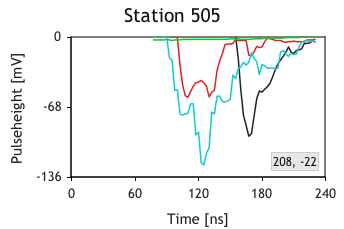
\includegraphics[scale=0.65]{Traces505}
    \caption{Ingewikkelde pulsvormen}
    \label{fig:Ingewikkelde-pulsvormen}
\end{figure}


\bigskip{}

In \figref{fig:Ingewikkelde-pulsvormen} valt het op dat de pulshoogte
van detector 2 (rood) kleiner is dan detector 1 (zwart).

\begin{minipage}[t]{1\columnwidth}%

\paragraph{Opdracht 4:}

Leg met de pulsintegraal (het pulsoppervlak) uit waarom er
waarschijnlijk evenveel deeltjes door detector 1 als door detector
2 zijn gegaan.

\begin{center}
    \rule{\textwidth}{0.3mm}\\
    \rule{\textwidth}{0.3mm}\\
    \rule{\textwidth}{0.3mm}\\
    \rule{\textwidth}{0.3mm}\\
\end{center}
\end{minipage}

\bigskip{}


In \figref{fig:Ingewikkelde-pulsvormen} valt het verder op dat detector
3 (groen) bijna geen puls geeft.

\begin{minipage}[t]{1\columnwidth}%

\paragraph{Opdracht 5:}

Verklaar waarom er binnen een station soms detectoren zijn
die een aantal deeltjes meten terwijl ander detectoren (bijna) niets
meten.

\begin{center}
    \rule{\textwidth}{0.3mm}\\
    \rule{\textwidth}{0.3mm}\\
    \rule{\textwidth}{0.3mm}\\
    \rule{\textwidth}{0.3mm}\\
\end{center}
\end{minipage}
\end{document}

\caption{Een signaal van een event in een \hisparc detector (station 501,
detector 4, 1 maart 2012 om 01:54:04).  Het signaal bestaat uit een
spanning uit een \pmt.  De (negatieve) spanning is recht evenredig met de
lichtintensiteit die op het venster van de \pmt valt.  In de staart van
het signaal zijn meerdere piekjes te zien.  Dit zijn deeltjes die op een
relatief laat tijdstip de detector bereikten.}
\label{fig:traces}
\end{figure}


\subsection{Pulshoogtehistogram}
\subsection{Drempels}

\section{Inregelen \pmts}


\begin{thebibliography}{9}
\bibitem{hamamatsu} Hamamatsu, \emph{Photomultiplier Tubes, Construction
and Operating Characteristics Connections to External Circuits} (1997).
\bibitem{9107B} ET Enterprises, Ltd., \emph{9107B series data sheet}
(2010), \url{http://my.et-enterprises.com/pdf/9107B.pdf}.
\end{thebibliography}

\end{document}
